\documentclass[aspectratio=169]{beamer}

\usepackage{beamerthemesplit}
\usepackage{amsmath}
\usepackage{amsfonts}
\usepackage{amssymb}
\usepackage{cancel}
\usepackage{bussproofs}
%% \usepackage{tkz-graph}

\makeatletter
\newcommand{\reallytiny}{\@setfontsize{\srcsize}{2pt}{2pt}}
\makeatother

\mode<presentation>
{
  \usetheme{AnnArbor}
  \usecolortheme{crane}
}

\usepackage[english]{babel}
\usepackage[latin1]{inputenc}
\usepackage{times}
\usepackage[T1]{fontenc}

\title{AI-DSL for Autonomous Interoperability}

\author{Nil Geisweiller}

\institute[SingularityNET OpenCog Foundations]
{
  \begin{center}
    SingularityNET \& OpenCog Foundations\\
    
\includegraphics[scale=0.32]{pics/snet_oc.png}
  \end{center}
}
          
\date[AI-DSL]

\begin{document}

\begin{frame}
  \maketitle
\end{frame}

\begin{frame}
  \frametitle{Example: Audio track $\rightarrow$ Music sheet}
  %% \begin{enumerate}
  %% \item Extract singing
  %% \item Speech-to-text
  %% \item Audio-to-midi
  %% \item Music sheet with lyrics
  %% \end{enumerate}
  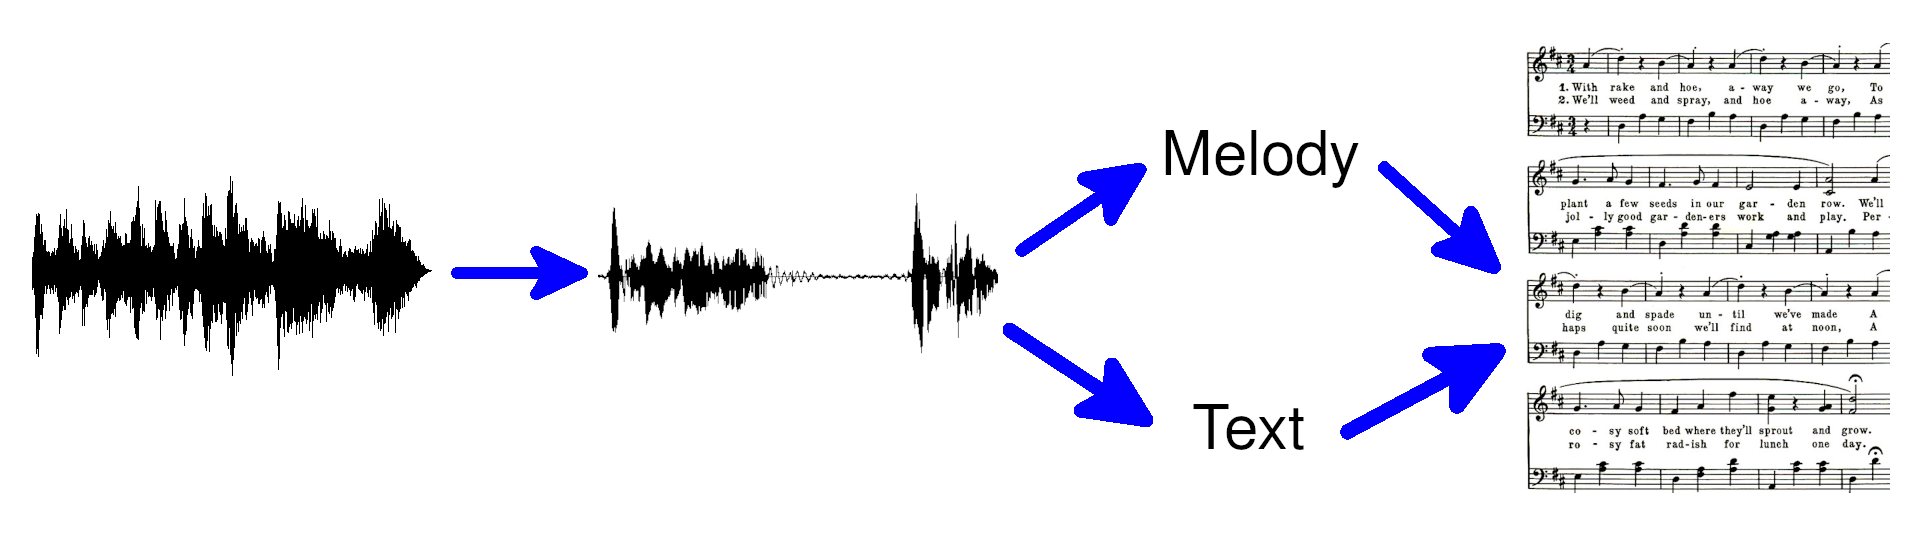
\includegraphics[scale=0.9]{pics/AI-inter-example.png}
\end{frame}

\begin{frame}
  \frametitle{Formal Specification of AIs}
  \begin{itemize}
  \item Solution:
    \begin{itemize}
    \item Formal description of AIs
    \end{itemize}

  \item Challenges:
    \begin{itemize}
    \item Writing formal description is tedious
    \item Requires concepts from real world
    \item Mismatches, sophisticated casting
    \item Performance evaluation, resource management
    \end{itemize}
  \end{itemize}
\end{frame}

\begin{frame}
  \frametitle{Writing Formal Specifications}
  \begin{itemize}
  \item Dependent Types: Idris, Agda, Liquid Haskell, etc.
  \item AIs can help too
    \begin{itemize}
    \item Code analysis
    \item Natural Language Processing of comments
    \end{itemize}
  \end{itemize}
\end{frame}

\begin{frame}
  \frametitle{Concepts from the real world}
  \begin{itemize}
  \item Ontologies
  \item Concept creation (AIs)
  \end{itemize}
\end{frame}

\begin{frame}
  \frametitle{Mismatches, sophisticated casting}
  \begin{itemize}
  \item<+-> $h : A \rightarrow C$
  \item<+-> We have 
    \begin{itemize}
    \item $f : A \rightarrow B$
    \item $g : B' \rightarrow C$
    \end{itemize}
  \item<+-> $c : B \rightarrow B'$
  \item<+-> $h = g . c . f$
  \end{itemize}
\end{frame}

\begin{frame}
  \frametitle{Performance evaluation, resource management}
  \begin{itemize}
  \item Probabilistic Model Checking
  \item Probabilistic Logic Networks
  \end{itemize}
\end{frame}

%% \begin{frame}
%%   \begin{enumerate}
%%   \item What?
%%     \begin{itemize}
%%     \item Provide \alert{formal} description of an AI
%%     \end{itemize}
%%   \item Why?
%%     \begin{itemize}
%%     \item Inform \alert{why} to use a certain AI
%%     \item Enable \alert{interoperability} between AIs
%%     \end{itemize}
%%   \item How?
%%     \begin{itemize}
%%     \item Dependent Types (Idris, AGDA, Coq, Liquid Haskell)
%%     \item Probabilistic Logic Networks (PLN), OpenCog Hyperion
%%     \item Natural Language Processing (NLP)!? (SingularityNET!?)
%%     \item $\dots$
%%     \end{itemize}
%%   \end{enumerate}
%% \end{frame}

%% \begin{frame}
%% * Braindump:

%%   - OpenCog:
  
%%     - MOSES:

%%       - infer type signature of the candidates to evolve given the
%%       fitness function, and define program spaces fulfilling such type
%%       signature.

%%       - Evolve candidates using search guided by reasoning, with a
%%       formalized local search and fitness function (SNET presentation)

%%     - Learning via Reasoning: OpenCog Pattern Miner, mining patterns
%%     fulfilling a specification.

%%     - Planning via Reasoning: discover plans (to control agent in env)
%%     provably probabilistically correct.

%%   - Magic Haskell.

%%   - Gluing mismatched programs. Need bridgers: bridgers need formal
%%   specification so they can be part of the network.
  
%%   - NLP: because often the only available specification is the
%%   documentation.

%%   - Why AI? Cause AI is hard. Either you think as hard as it is, or
%%   you go out there a get the knowledge.

%%   - SampleLink: what the magic? Reasoning.

%%   - Likely needs ontology of concepts (types) to make the life of the
%%   developer easier.

%%   - Performance evaluation for more informative specification.
%% \end{frame}

%% \begin{frame}
%%   Code reuse, see

%%   https://vimeo.com/131194141
%%   https://en.wikipedia.org/wiki/Code_reuse
%%   https://www.perforce.com/blog/qac/challenge-code-reuse-and-how-reuse-code-effectively
%% \end{frame}

%% \begin{frame}

%%   - RepresentationalLanguage     -- Formal grammar to represent candidates
  
%%   Fitness -> InitialPopulation -> OptimizedPopulation

%%   Fitness -> ResourceManagement -> Termination -> InitialPopulation -> OptimizedPopulation

%%   Fitness -> ResourceManagement -> BackgroundKnowledge -> Termination -> InitialPopulation -> OptimizedPopulation

%% - rp : RepresentationalLanguage

%% - Candidate = Instantiate rp
%% - Fitness = Candidate -> Float
%% - InitialPopulation = Set Candidate
%% - OptimizedPopulation = Multimap Float Candidate
%% - Termination -- Termination criteria, may depend on the state of the learner!
%% - ResourceManagement -- How much time and space resources to allocate
%% - BackgroundKnowledge -- Any knowledge that could be useful (domain specific, meta-heuristics, etc). Requires a common language.

%% \end{frame}

%% \begin{frame}
%%   \frametitle{More detailed example: MOSES}
%%   \center{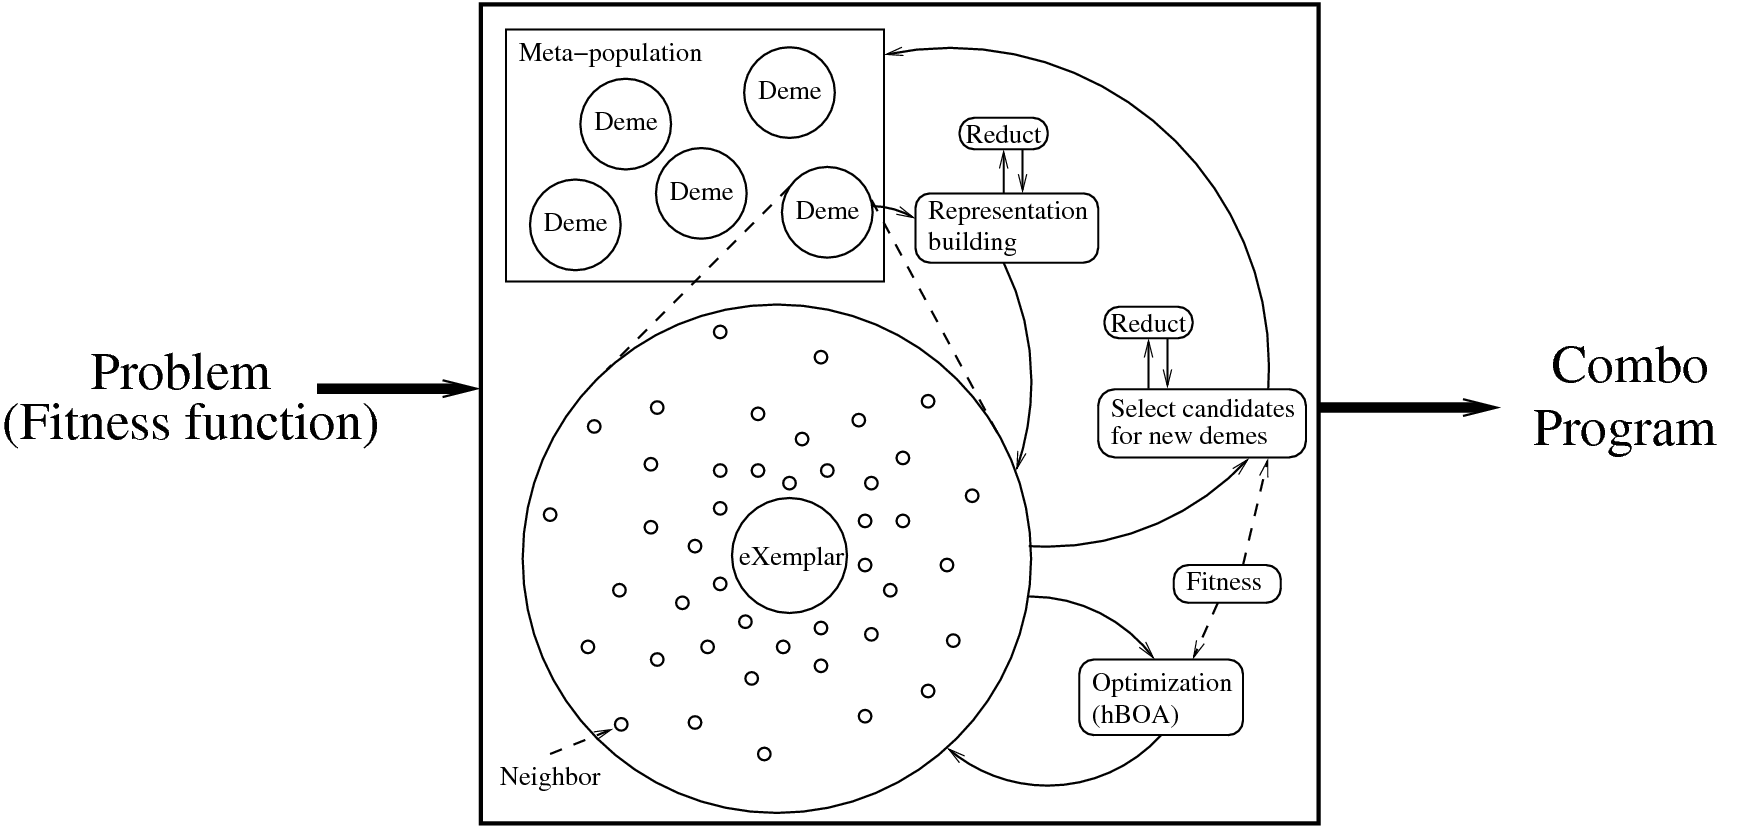
\includegraphics[scale=0.23]{pics/MOSESSumDetails.png}}
%% \end{frame}

\begin{frame}
  \frametitle{Evolutionary Programing: Examples of properties}
  \begin{itemize}
  \item Deterministic Hillclimbing : (f : Fitness) $\rightarrow$ unimodal(f) $\rightarrow$ converge(f)
  \item Stochastic Hillclimbing : (f : Fitness) $\rightarrow$
    multimodal(f) $\rightarrow$ avg-exp-converge(f)
  \item BOA : (f : Fitness) $\rightarrow$ decomposable(f) $\rightarrow$ avg-subexp-converge(f)
  %% \item BOA : \{f : Fitness\} $\rightarrow$ decomposable(f)
  %%   $\rightarrow$ deceptive(f) $\rightarrow$ avg-subexp-converge(f)
  \end{itemize}

  $$\Downarrow$$
  
  \center{\alert{Probability monads?}}

\end{frame}

\begin{frame}

Related bibliography:

{\footnotesize
  \begin{enumerate}
  \item TF-Coder: Program Synthesis for Tensor Manipulations
    https://arxiv.org/pdf/2003.09040.pdf

  \item C2S: Translating Natural Language Comments to FormalProgram Specifications
    https://www.cs.purdue.edu/homes/lintan/publications/c2s-fse20.pdf

  \item Formal Specification for Deep Neural Networks
    https://www2.eecs.berkeley.edu/Pubs/TechRpts/2018/EECS-2018-25.pdf

  \item An epistemic approach to the formal specification of statistical
    machine learning
    https://link.springer.com/article/10.1007/s10270-020-00825-2

  \item CAMUS: A Framework to Build Formal Specifications for Deep Perception
    Systems Using Simulators
    https://arxiv.org/abs/1911.10735

  \item VerifAI is a software toolkit for the formal design and analysis of
    systems that include artificial intelligence (AI) and machine learning
    (ML) components
    https://github.com/BerkeleyLearnVerify/VerifAI

  \item LTL and Beyond: Formal Languages for Reward Function Specification in
    Reinforcement Learning
    https://www.ijcai.org/Proceedings/2019/840

  \item Developing Bug-Free Machine Learning Systems With Formal Mathematics
    https://arxiv.org/abs/1706.08605

  \item Verified Stack-Based Genetic Programming via Dependent Types
    https://cogsys.uni-bamberg.de/events/aaip11/accepted/diehl.pdf
  \end{enumerate}
}

\end{frame}

\begin{frame}[fragile]

{\tiny
\begin{verbatim}
Split MOSES into 3 modules:

Vectorize -- Turn syntax tree into vector space (program subspace)
Optimize vector space -- Find good vector candidate
Meta-optimize -- Discover regularities in the vector space

Example: MOSES, evolve syntax trees, call external AI for the
optimization step in vector space.

* MOSES (very abstract) type signature:

moses : Fitness -> Population -> Population

data Candidate = ... -- Syntax tree
type Fitness = Candidate -> Float
type Population = Map Candidate Float

* Optimize Vector Space (very abstract) type signature:

VecFitness -> (Vector Float) -> VecPopulation
type VecFitness = Vector Float -> Float
type VecPopulation = Map (Vector Float) Float

* Meta-optimize (very abstract) type signature:

type OptimizationRecord = Map (Vector Float) Float = VecPopulation
data FitnessEstimate = ... -- Probabilistic model
moptimize : OptimizationRecord -> FitnessEstimate

Run backward from the fitness to the candidates.
\end{verbatim}
}

%%   TODO:

%%   moses_rec : Fitness -> Population -> Termination -> Population
%%   moses_rec f is t = moses (select is)
%%     fold (\i -> vecopt (f . s) (v i)) (select is) ...

\end{frame}

\begin{frame}[fragile]

{\tiny
\begin{verbatim}
* Putting it all together:

f : Fitness
v : Vectorize
s : Symbolize

vecopt : VecFitness -> (Vector Float) -> VecPopulation
vecopt_rec : VecFitness -> (Vector Float) -> Termination -> VecPopulation

i : Candidate -- Initial candidate
moses f i = vecopt_rec (f . s) (v i) t
  where s, v, t ...

vf : VecFitness
fe : FitnessEstimate
vi : Vector Float
t : Termination
vecopt_rec vf fe vi t = (union sols (vecopt_rec vf nfe (decrease t)))
  where sols = (vecopt vf vi),
        new_fe = (join (moptimize sols) fe (select sols)),
        join = ... -- merge 2 fitness estimates  
\end{verbatim}
}

\end{frame}

\end{document}
